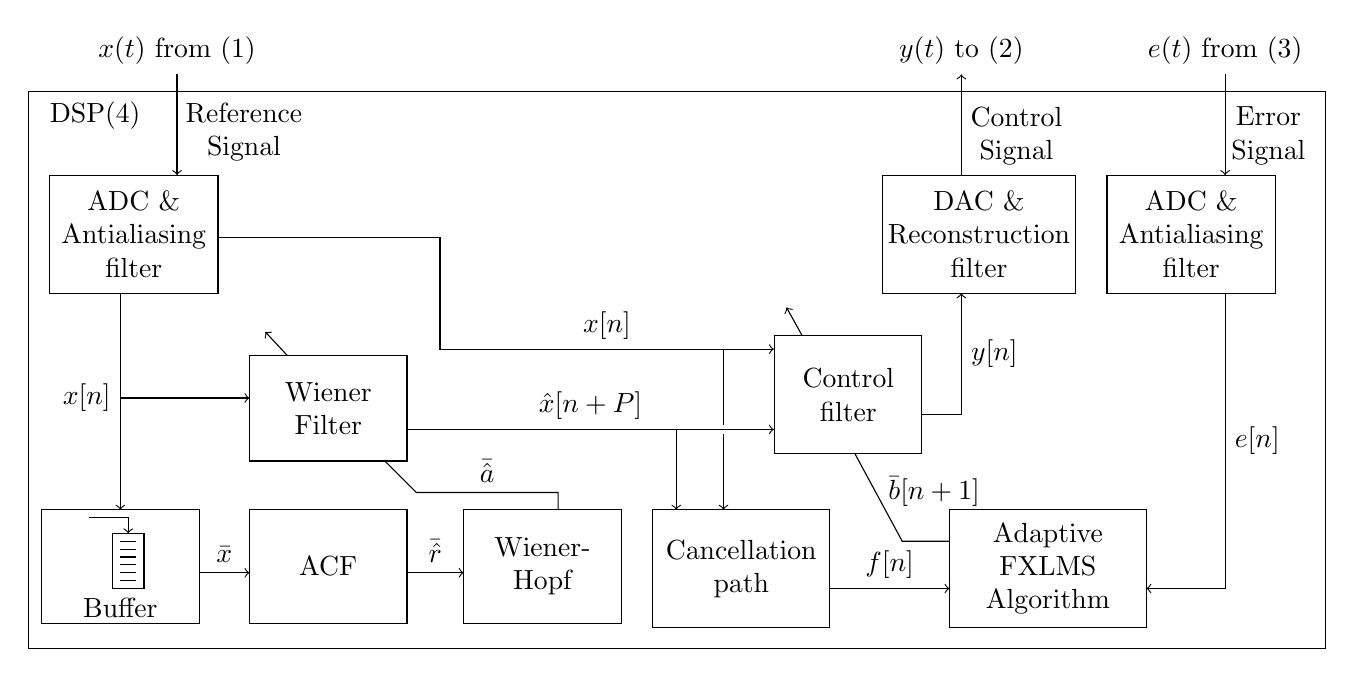
\begin{tikzpicture}
\draw  (-6.96,-2.17) rectangle node[text width=2cm,align=center] {ADC \& Antialiasing filter} (-4.82,-3.67);
\draw  (0.7,-6.42) rectangle node[text width=2.5cm,align=center] {Cancellation \\ path}(2.95,-7.92);
\draw  (4.47,-6.42) rectangle node[text width=2.5cm,align=center] {Adaptive FXLMS Algorithm} (6.97,-7.92);

\draw  (2.25,-4.21) rectangle node[text width=1.5cm,align=center,fill=white] {Control filter} (4.12,-5.71);
\draw  (3.62,-2.17) rectangle node[text width=2.5cm,align=center] {DAC \& \\ Reconstruction filter}(6.07,-3.67);
\draw  (6.47,-2.17) rectangle node[text width=2cm,align=center] {ADC \& Antialiasing filter}(8.61,-3.67);

\draw  (-7.23,-1.11) rectangle (9.25,-8.18);
\node at (-6.38,-1.41) {DSP(4)};
\node [text width=2cm,align=center] at (-4.49,-1.62) {Reference Signal};

\draw[->] (2.95,-7.42) -- node[above]{$f[n]$} (4.47,-7.42);

\draw[->] (7.97,-3.67) -- node[right]{$e[n]$} (7.97,-7.42)  -- (6.97,-7.42);

\draw [->](7.97,-0.89) node[above]{$e(t)$ from (3)} -- (7.97,-2.17) ;
\draw [->](4.62,-2.17)  --  (4.62,-0.89) node[above]{$y(t)$ to (2)};




\draw[->] (4.12,-5.21) -- (4.62,-5.21) --node[right]{$y[n]$} (4.62,-3.67);
\draw [->](-5.34,-0.89) node[above]{$x(t)$ from (1)} -- (-5.34,-2.17);
\node [text width=2cm,align=center] at (5.32,-1.67) {Control Signal};
\node [text width=1.5cm,align=center] at (8.52,-1.67) {Error Signal};

\draw (4.47,-6.82) -- (3.87,-6.82) --node[above=2.25,right]{$\bar{b}[n+1]$} (3.27,-5.71);
\draw [->](2.6,-4.21) -- (2.4,-3.85);


%% Boxes
\draw  (-4.42,-5.8) rectangle node[text width=2cm,align=center] {Wiener Filter}(-2.42,-4.46);
\draw  (-2.42,-6.42) rectangle node[text width=2cm,align=center] {ACF}(-4.42,-7.86);
\draw  (-5.06,-6.42) rectangle node[text width=2cm,align=center,below=8] {Buffer}(-7.06,-7.86);
\draw  (-1.7,-6.42) rectangle node[text width=1.5cm,align=center] {Wiener- Hopf}(0.3,-7.86);



%%Buffer
\draw (-5.76,-7.42) node (v1) {} -- (-6.16,-7.42) -- (-6.16,-6.72) -- (-5.76,-6.72) -- (-5.76,-7.42);
\draw (-6.06,-6.82) -- (-5.86,-6.82);
\draw (-6.06,-6.92) -- (-5.86,-6.92);
\draw (-6.06,-7.02) -- (-5.86,-7.02);
\draw (-6.06,-7.12) -- (-5.86,-7.12);
\draw (-6.06,-7.22) -- (-5.86,-7.22);
\draw (-6.06,-7.32) -- (-5.86,-7.32);
\draw [->](-6.46,-6.52) -- (-5.96,-6.52) -- (-5.96,-6.72);


%% Lines
\draw [->](-5.06,-7.22) -- node[above]{$\bar{x}$} (-4.42,-7.22);
\draw [->](-2.42,-7.22) -- node[above]{$\bar{\hat{r}}$}(-1.7,-7.22);
\draw (-0.5,-6.42) -- (-0.5,-6.2) -- node[above]{$\bar{\hat{a}}$} (-2.3,-6.2) -- (-2.7,-5.8);


\draw [->](-3.94,-4.46) -- (-4.22,-4.16);
\draw [->](-6.06,-5)  node[left]{$x[n]$} -- (-4.42,-5);
\draw [->](-6.06,-3.68) -- (-6.06,-6.42);
\draw [->](-2.42,-5.4) --  node[above]{$\hat{x}[n+P]$}(2.24,-5.4);

\draw [->](-4.82,-2.96) -- (-4.56,-2.96) -- (-2,-2.96) -- (-2,-4.38) -- node[above]{$x[n]$} (2.24,-4.38);
\draw (1.6,-4.38) -- (1.6,-5.34);
\draw [->](1.6,-5.46) -- (1.6,-6.42);
\draw [->](1,-5.4) -- (1,-6.42);
\end{tikzpicture}